\documentclass[oneside, a4paper, 12pt]{book}
\usepackage[ngerman]{babel}
\usepackage{graphicx}
\usepackage{calc}
\usepackage{fancyvrb}
\pagestyle{empty}
\usepackage[utf8]{inputenc}
\usepackage{array}
\inputencoding{latin1}
\usepackage[absolute,showboxes]{textpos}

%\usepackage[absolute]{textpos}
\usepackage[]{eso-pic}[2002/11/16]

\usepackage{fancybox} % fuer Oval...

%\usepackage{showframe}


\setlength{\tabcolsep}{0.2cm}
\setlength{\topmargin}{1cm}
\setlength{\parindent}{0pt}

\newlength{\Rand}
\setlength{\Rand}{\oddsidemargin + \hoffset + 1in}

\begin{document}
\fontfamily{phv}\selectfont
\textblockorigin{0cm}{0cm}

\newlength{\Logo}
\setlength{\Logo}{210mm-60mm}
\begin{textblock*}{\Logo}(30mm,30mm)%

\includegraphics[width=\Logo]{pcars-main.png}
\end{textblock*}

\begin{textblock*}{\Logo}(30mm,150mm)%
\begin{center}\Huge{pCars Tracks 21. May 2015}\end{center}
\end{textblock*}

\begin{textblock*}{\Logo}(30mm,165mm)%
\begin{center}\tt\large{https://github.com/wwwutz/pCars-Tracks}\end{center}
\end{textblock*}


\begin{textblock*}{30mm}(0mm,0mm)%

\includegraphics[width=30mm]{LG/2015-05-20_00094.png}
\end{textblock*}
\begin{textblock*}{30mm}(30mm,0mm)%

\includegraphics[width=30mm]{LG/2015-05-20_00086.png}
\end{textblock*}
\begin{textblock*}{30mm}(60mm,0mm)%

\includegraphics[width=30mm]{LG/2015-05-20_00072.png}
\end{textblock*}
\begin{textblock*}{30mm}(90mm,0mm)%

\includegraphics[width=30mm]{LG/2015-05-20_00076.png}
\end{textblock*}
\begin{textblock*}{30mm}(120mm,0mm)%

\includegraphics[width=30mm]{LG/2015-05-20_00089.png}
\end{textblock*}
\begin{textblock*}{30mm}(150mm,0mm)%

\includegraphics[width=30mm]{LG/2015-05-20_00074.png}
\end{textblock*}
\begin{textblock*}{30mm}(180mm,0mm)%

\includegraphics[width=30mm]{LG/2015-05-20_00092.png}
\end{textblock*}
\begin{textblock*}{30mm}(0mm,30mm)%

\includegraphics[width=30mm]{LG/2015-05-20_00080.png}
\end{textblock*}
\begin{textblock*}{30mm}(180mm,30mm)%

\includegraphics[width=30mm]{LG/2015-05-20_00091.png}
\end{textblock*}
\begin{textblock*}{30mm}(0mm,60mm)%

\includegraphics[width=30mm]{LG/2015-05-20_00097.png}
\end{textblock*}
\begin{textblock*}{30mm}(180mm,60mm)%

\includegraphics[width=30mm]{LG/2015-05-20_00081.png}
\end{textblock*}
\begin{textblock*}{30mm}(0mm,90mm)%

\includegraphics[width=30mm]{LG/2015-05-20_00087.png}
\end{textblock*}
\begin{textblock*}{30mm}(180mm,90mm)%

\includegraphics[width=30mm]{LG/2015-05-20_00083.png}
\end{textblock*}
\begin{textblock*}{30mm}(0mm,120mm)%

\includegraphics[width=30mm]{LG/2015-05-20_00085.png}
\end{textblock*}
\begin{textblock*}{30mm}(180mm,120mm)%

\includegraphics[width=30mm]{LG/2015-05-20_00079.png}
\end{textblock*}
\begin{textblock*}{30mm}(30mm,150mm)%

\includegraphics[width=30mm]{LG/2015-05-20_00100.png}
\end{textblock*}
\begin{textblock*}{30mm}(90mm,150mm)%

\includegraphics[width=30mm]{LG/2015-05-20_00096.png}
\end{textblock*}
\begin{textblock*}{30mm}(150mm,150mm)%

\includegraphics[width=30mm]{LG/2015-05-20_00099.png}
\end{textblock*}
\begin{textblock*}{30mm}(0mm,180mm)%
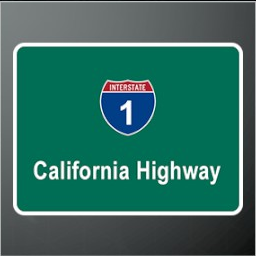
\includegraphics[width=30mm]{LG/2015-05-20_00077.png}
\end{textblock*}
\begin{textblock*}{30mm}(60mm,180mm)%

\includegraphics[width=30mm]{LG/2015-05-20_00098.png}
\end{textblock*}
\begin{textblock*}{30mm}(120mm,180mm)%

\includegraphics[width=30mm]{LG/2015-05-20_00075.png}
\end{textblock*}
\begin{textblock*}{30mm}(180mm,180mm)%
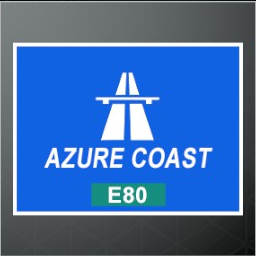
\includegraphics[width=30mm]{LG/2015-05-20_00073.png}
\end{textblock*}
\begin{textblock*}{30mm}(30mm,210mm)%

\includegraphics[width=30mm]{LG/2015-05-20_00082.png}
\end{textblock*}
\begin{textblock*}{30mm}(90mm,210mm)%

\includegraphics[width=30mm]{LG/2015-05-20_00078.png}
\end{textblock*}
\begin{textblock*}{30mm}(150mm,210mm)%

\includegraphics[width=30mm]{LG/2015-05-20_00095.png}
\end{textblock*}
\begin{textblock*}{30mm}(0mm,240mm)%

\includegraphics[width=30mm]{LG/2015-05-20_00088.png}
\end{textblock*}
\begin{textblock*}{30mm}(60mm,240mm)%

\includegraphics[width=30mm]{LG/2015-05-20_00093.png}
\end{textblock*}
\begin{textblock*}{30mm}(120mm,240mm)%

\includegraphics[width=30mm]{LG/2015-05-20_00090.png}
\end{textblock*}
\begin{textblock*}{30mm}(180mm,240mm)%

\includegraphics[width=30mm]{LG/2015-05-20_00084.png}
\end{textblock*}
;

%\null\newpage



\end{document}
